\documentclass[11pt]{beamer}
\usepackage[utf8]{inputenc}
\usepackage[T1]{fontenc}
\usepackage{lmodern}
\usetheme{Marburg}
\usecolortheme{crane}
\begin{document}
	\author{A R Bathri Narayanan}
	\title{Search on Superconducting Qubits}
	\subtitle{International Young Quantum Meet 2024}
	%\logo{}
	\institute{UM-DAE Centre for Excellence in Basic Sciences}
	\date{September 18, 2024}
	\subject{}
	%\setbeamercovered{transparent}
	%\setbeamertemplate{navigation symbols}{}
	\begin{frame}[plain]
		\maketitle
	\end{frame}
	
	\begin{frame}
		\frametitle{Introduction to the talk}
		Qubits can be realised in a lot of ways, examples include
		\begin{enumerate}
			\item  Ion trap quantum computing
			\item NMR quantum computing
			\item Optical photon quantum computing to name a few.
		\end{enumerate}
	My talk will be focused more on Superconducting qubits and applying it to model a theoretical problem.
	\end{frame}
	
		\begin{frame}
		\frametitle{How do you build Superconducting Qubits}
		By using so called "Artificial atoms". You cool a LC circuit to the material's critical temperature, into it's superconducting phase.\\
		\begin{center}
		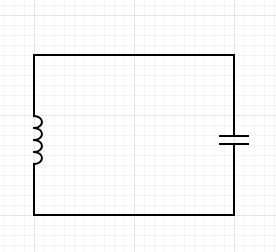
\includegraphics[width=3 cm]{sc1.png}
		\end{center}
		Where,
		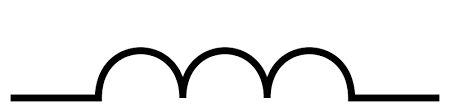
\includegraphics[width=1 cm]{sc2.png} means Inductor and 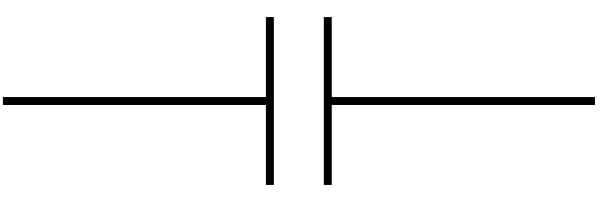
\includegraphics[width=1 cm]{sc3.jpg} means Capacitor. The Hamiltonian of this circuit is given by
		\[H=\frac{\hat{Q}}{2C}+\frac{\hat{\Phi}}{2L}=\hbar\omega(aa^{\dagger}+\frac{1}{2})\]
		\end{frame}
		
				\begin{frame}
			\frametitle{Issues with simple superconducting qubits}
			Energy levels of the circuit mimic a linear Harmonic oscillator
			\begin{center}
			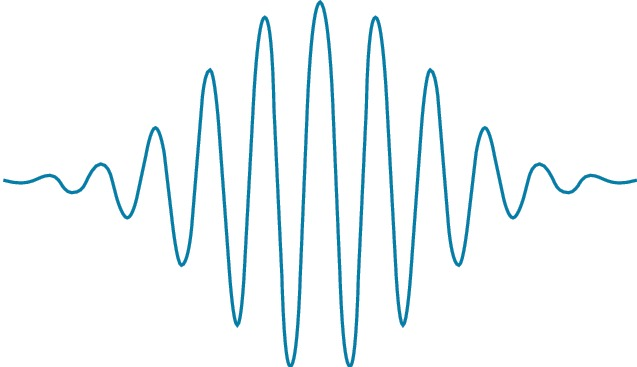
\includegraphics[width=2 cm]{sc5.jpg}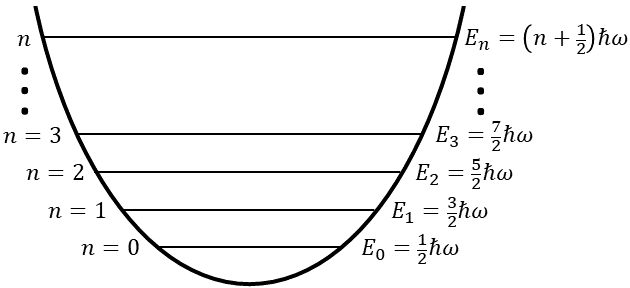
\includegraphics[width=5 cm]{sc4.png}
			\end{center}
			This can't be an ideal two qubit system as all energy levels are equally spaced. But how do we modify the energy levels?\\
			Enter \textbf{Josephson Junctions} !!
			\begin{center}
				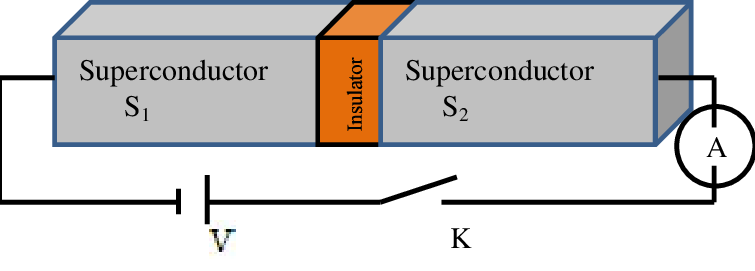
\includegraphics[width=5 cm]{sc6.png}
			\end{center}

		\end{frame}
	
		\begin{frame}
		\frametitle{How can you modify Superconducting Qubits (Josephson Junctions and dc-SQUIDs)}
		Josephson Junctions are represented by 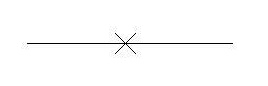
\includegraphics[width=1 cm]{sc7.png}. I am not focusing more on the derivation of V, I and L of Josephson Junctions, I just mention it here. Interested can refer to Feynman lectures volume 3 last chapter.
		\[V_J=\frac{\Phi_0}{2\pi}\frac{d\varphi_J}{dt}\]
		\[I_J=I_c sin \varphi_J\]
		\[L_J=\frac{\phi_J}{I_csin(2\pi\phi_J/\phi_0)}=\frac{\phi_0\varphi_J}{2\pi I_c sin\varphi_J}\]
		The circuit can be drawn like\\
		\begin{center}
			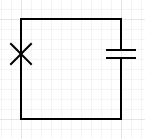
\includegraphics[width=2cm]{sc8.png}
		\end{center}
	

	\end{frame}
	
	\begin{frame}
		\frametitle{Analog gravity using superconducting qubits}
		We construct an infinite circuit like
		\begin{center}
			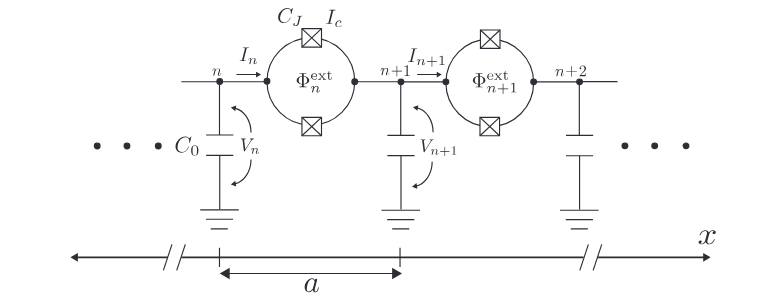
\includegraphics[width=8 cm]{sc9.png}
		\end{center}
		Now, we apply Kirchoff law and Faraday's law as
		\[I_n - I_{n+1}=\frac{dQ_{n+1}}{dt}\]
		\[V_n-V_{n+1}=\frac{\Phi_0}{2\pi}\frac{d\varphi_{Jn}}{dt}\]
	\end{frame}
	
		\begin{frame}
		\frametitle{Obtaining the equation of motion}
Plugging in the formulas obtained for Josephson junctions, we can obtain the current entering the nth unit cell as
\[I_n=2 C_J \frac{\Phi_0}{2\pi}\frac{d^2\varphi_{Jn}}{dt^2}+2I_ccos\bigg(\frac{\pi \Phi^{ext}_n}{\Phi_0}\bigg)sin\varphi_{Jn}\]
Applying $\varphi_{Jn}$=$\varphi_{n}$-$\varphi_{n+1}$ and plugging the above in the $V_n$ equation, we obtain
\[(C_0+4C_J)\bigg(\frac{\Phi_0}{2\pi}\bigg)^2\frac{d^2\varphi_{n}}{dt^2}-2C_J\bigg(\frac{\Phi_0}{2\pi}\bigg)^2\bigg( \frac{d^2\varphi_{n-1}}{dt^2}+\frac{d^2\varphi_{n+1}}{dt^2}  \bigg)\]
\[=-2E_Jcos\bigg(\frac{\pi \Phi^{ext}_n}{\Phi_0}\bigg)sin(\varphi_{n}-\varphi_{n+1})+2E_Jcos\bigg(\frac{\pi \Phi^{ext}_{n-1}}{\Phi_0}\bigg)sin(\varphi_{n-1}-\varphi_{n})\]
	\end{frame}
	
	\begin{frame}
		\frametitle{Obtaining the EM phase speed}
We can guess the Lagrangian, and eventually the Hamiltonian, which is nothing but
\[H=\int_{-\infty}^{\infty}dx\bigg[\bigg(\frac{2\pi}{\Phi_0}\bigg)^2\frac{p^2}{2\mathcal{C}}+E_Jacos\bigg(\frac{\pi \Phi^{ext}}{\Phi_0}\bigg)\bigg(\frac{\partial\varphi}{\partial x}\bigg)^2\bigg]\]
Of course we make a few approximations like the continuum approximation, neglecting the Josephson junction capacitance term. 
We get the following wave equation
\[\frac{\partial^2\varphi}{\partial t^2}=\frac{\partial}{\partial x}\bigg(c^2\frac{\partial \varphi}{\partial x}\bigg),c=\frac{1}{\sqrt{\mathcal{L}\mathcal{C}}}\]
Where,
\[\mathcal{C}=C_0/a,\mathcal{L}=\frac{\Phi_0}{4\pi I_ca}sec\bigg(\frac{\pi \Phi^{ext}}{\Phi_0}\bigg)\]
	\end{frame}
	
		\begin{frame}
		\frametitle{Getting the covariant wave equation}
Now, we transform as x'=x-ut, t'=t, the wave equation becomes 
\[\bigg(-\frac{\partial^2}{\partial t^2}+2u\frac{\partial^2}{\partial x\partial t}+\frac{\partial}{\partial x}\big(c^2-u^2\big)\frac{\partial}{\partial x}\bigg)\varphi=0=\frac{1}{\sqrt{-g}}\partial_\mu(\sqrt{-g}g^{\mu\nu}\partial_\nu\varphi)\]
Where,
\[ g^{\mu\nu}=\frac{1}{c}
\begin{pmatrix}
	-1 & u \\
	u & c^2-u^2 
\end{pmatrix}
\]
We finally take the Hawking temperature
\[T_H=\frac{\hbar}{2\pi k_B}\bigg|\frac{\partial c}{\partial x}\bigg|_{x_h}\]
And plug in the respective values to get an estimate (for $\bigg|\frac{\partial c}{\partial x}\bigg|_{x_h}$$\approx$0.01$c_0$/a, $C_0$=1$\mu$ F, $I_c$=5$\mu$A, $T_h$= 70 mK)
 
	\end{frame}
	
		\begin{frame}
		\frametitle{Conclusions and future directions}
		So in this talk, we have discussed about
		\begin{enumerate}
			\item A brief introduction to Superconducting qubits
			\item  Construction of superconducting qubits
			\item  A brief application of superconducting qubits in Analogue Gravity and Hawking radiation.
			\end{enumerate}
			
			In the future I have planned for
			\begin{enumerate}
				\item Trying to model the Unruh effect by following the footsteps of Blencowe
				\item Trying to study on Current mirror qubits as introduced by Kitaev.
			\end{enumerate}
	\end{frame}
	
			\begin{frame}
		\frametitle{Acknowledgements}
		I would like to thank the following people for guiding me in the right direction
		\begin{enumerate}
			\item Prof. R Nagarajan, Emeritus professor, UM-DAE Centre for Excellence in Basic Sciences
			\item Prof. Sudhir Ranjan Jain, Adjunct faculty, UM-DAE Centre for Excellence in Basic Sciences
			\item  Prof. Amarendra Kumar Sarma, Professor, IIT Guwahati
			\item Prof. Ujjwal Sen, Professor-H, Harish-Chandra Research institute
		\end{enumerate}
	\end{frame}
	
	\begin{frame}
		\begin{center}
			\LARGE\textbf{Thank You !!} \\
			Any doubts : arbathri.narayanan@cbs.ac.in
		\end{center}
	
	\end{frame}
\end{document}